%Dokumentklasse
\documentclass[a4paper,12pt,makeidx,twoside,openright,numbers=noenddot]{scrreprt}
\usepackage[left=3cm, right=2cm, bottom=2.5cm, top=3cm]{geometry}		% Formatierung der Seitenränder
%\usepackage[onehalfspacing]{setspace}							        % verwendet für größeren Zeilenabstand

% ============= Packages =============

% Dokumentinformationen


\usepackage[
	pdftitle={},
	pdfsubject={},
	pdfauthor={},
	pdfkeywords={}
]{hyperref}

%could useful for project work to stop the new page clearpage and cleardoublepage must be deleted
%\makeatletter
%\renewcommand\chapter{\thispagestyle{plain}%
%\global\@topnum\z@
%\@afterindentfalse
%\secdef\@chapter\@schapter}
%\makeatother 

\usepackage[utf8]{inputenc}
%\usepackage[ngerman]{babel}
\usepackage[british,UKenglish,USenglish,english,american]{babel}
\usepackage[T1]{fontenc}
\usepackage{units}
\usepackage{pdfpages}
\usepackage{listings}
\usepackage{svg}					% Zur Einbindung von scalable vector graphics
\usepackage{subcaption}				% Zum Einbinden von Untergrafiken
\usepackage[gen]{eurosym}			% Zur Verwendung des Eurozeichens
\usepackage{amssymb}
\usepackage{graphicx}
\graphicspath{{img/}}				
\usepackage{fancyhdr}				% Style Package für's Seitenlayout
\usepackage{color}					% anpassen von Farben
\usepackage{microtype} 				% schönerer Blocksatz!
\usepackage{calc}  					
\usepackage{enumitem}				% zb für align der description
\usepackage[font=small,labelfont=bf]{caption}
\usepackage[printonlyused]{acronym}	% für Abkürzungen
\usepackage{multicol}
\usepackage{booktabs}
\usepackage{textcomp}
\usepackage{listings}				% Einbindung von Code in LateX
\usepackage{setspace}
\usepackage{threeparttable} 		% für Fußnoten innerhalb einer Tabelle
\usepackage{placeins}


% CODE PLUGIN!!
%\usepackage{minted}

% verschiedene Schriftarten
%\usepackage{times} 				% times font
%\usepackage{palatino}			 	% Palatino font
\usepackage{lmodern}				% Lmodern sans und serif
%\usepackage{libertine}				% Linux Libertine und Biolinum

%\usepackage{fontspec}				% Nutzen in Kombination mit LuaLaTeX, um Systemschriften einzubinden
%\setmainfont{Georgia}				% beispielsweise Georgia, aber auch jede andere Schrift, die auf dem PC vorhanden ist


% zusätzliche Schriftzeichen der American Mathematical Society
\usepackage{amsfonts}
\usepackage{amsmath}



\usepackage[numbers, comma]{natbib}		% Einstellung des Zitierstils
%\bibliographystyle{myabbrvnat}			% Angepasster Stil für deutsche Sprache



\setcounter{secnumdepth}{3}				% Nummerierungsebene anpassen -> 3 = subsubsection werden nummeriert
\setcounter{tocdepth}{2}   				% gliederungsebenen im Inhaltsverzeichnis -> erstmal nur zur übersicht was nicht vergessen werden darf

\definecolor{deepblue}{rgb}{0,0,0.5}
\definecolor{deepred}{rgb}{0.6,0,0}
\definecolor{deepgreen}{rgb}{0,0.5,0}


% ============= Kopf- und Fußzeile =============
\pagestyle{fancy}

%% Formatierung der Kopf- und Fußzeile
\fancyhead{}
\fancyhead[RO,LE]{\thepage}
\fancyhead[RE]{\leftmark}
\fancyhead[LO]{\rightmark}
%%
\fancyfoot{}

\renewcommand{\headrulewidth}{0.4pt}		% Bei zweiseitigem Dokument ausschließlich Linie in Kopfzeile
\renewcommand{\chaptermark}[1]{\markboth{\thechapter\ #1}{}}
\renewcommand{\sectionmark}[1]{\markright{\thesection\ #1}}

% ============= Package Einstellungen & Sonstiges ============= 
% Besondere Trennungen
\hyphenation{Um-ge-bungs-tem-pe-ra-tur Um-ge-bungs-tem-pe-ra-tur-en Rauch-gas-tem-pe-ra-tur Aus-tritts-tem-pe-ra-tur}

% Einstellung wie Code innerhalb der Arbeit gesetzt werden soll:
\lstdefinestyle{Style}{
	columns=flexible,
	basicstyle=\ttfamily}
\lstset{ 
	backgroundcolor=\color{white},   % choose the background color; you must add \usepackage{color} or \usepackage{xcolor}; should come as last argument
	basicstyle=\footnotesize,        % the size of the fonts that are used for the code
	breakatwhitespace=false,         % sets if automatic breaks should only happen at whitespace
	breaklines=true,                 % sets automatic line breaking
	captionpos=none,                 % sets the caption-position to bottom
	commentstyle=\color{deepblue},   % comment style
	deletekeywords={...},            % if you want to delete keywords from the given language
	escapeinside={\%*}{*)},          % if you want to add LaTeX within your code
	extendedchars=true,              % lets you use non-ASCII characters; for 8-bits encodings only, does not work with UTF-8
	firstnumber=1,               	 % start line enumeration with line 1000
	frame=single,	                 % adds a frame around the code
	keepspaces=true,                 % keeps spaces in text, useful for keeping indentation of code (possibly needs columns=flexible)
	keywordstyle=\color{blue},       % keyword style
	language=Python,                 % the language of the code
	morekeywords={*,...},            % if you want to add more keywords to the set
	numbers=left,                    % where to put the line-numbers; possible values are (none, left, right)
	numbersep=5pt,                   % how far the line-numbers are from the code
	emphstyle=\color{deepred},
	%numberstyle=\tiny\color{mygray}, % the style that is used for the line-numbers
	rulecolor=\color{black},         % if not set, the frame-color may be changed on line-breaks within not-black text (e.g. comments (green here))
	showspaces=false,                % show spaces everywhere adding particular underscores; it overrides 'showstringspaces'
	showstringspaces=false,          % underline spaces within strings only
	showtabs=false,                  % show tabs within strings adding particular underscores
	stepnumber=2,                    % the step between two line-numbers. If it's 1, each line will be numbered
	stringstyle=\color{deepgreen},     % string literal style
	tabsize=2,	                   	 % sets default tabsize to 2 spaces
	title=\lstname                   % show the filename of files included with \lstinputlisting; also try caption instead of title
}

% nicht einrücken nach Absatz
\setlength{\parindent}{0pt}
\usepackage{parskip}		 			% verhindert einrücken und setzt einen kleinen Absatz

\renewcommand{\arraystretch}{1.2}		% Abstand innerhalb der Tabellen einstellen

\newcommand*{\mytitle}{Disease Detection in Sugar beet Plant Leaves} % Titel
\newcommand*{\myinstitute}{Department Lippstadt 2} % Institut


\newcommand*{\myauthor}{Olaniyi Bayonle Alao} % Autoren
\newcommand*{\myreporttype}{Project Work} % Bericht-Typ
\newcommand*{\mygraduation}{Bachelor of Engineering} % Vollständige Anschrift



\newcommand*{\firstexaminer}{Prof. Dr. Stefan Henkler} % Ort
\newcommand*{\secondexaminer}{Dipl.-Wirt.-inf. Kristian Rother} % Ort
\newcommand*{\mydate}{\today} % Datum


% ============= Dokumentbeginn =============

\begin{document}

% Seiten ohne Kopf- und Fußzeile sowie Seitenzahl
\pagestyle{empty}

\begin{center}
\begin{tabular}{p{\textwidth}}

\begin{center}
	
\includegraphics[scale=0.12]{HSHL_Logo_horizontal_RGB_blue_green_mit-Schutzraum_ENG.jpg}
\end{center}


\\

\begin{center}
\LARGE{\textbf{
\mytitle\\[1cm]
}}
\end{center}

\\


\begin{center}
\large{\myinstitute\\}

\end{center}

\\\\

\begin{center}
\textbf{\Large{\myreporttype}}
\end{center}


%\begin{center}
%for optainment of the degree of\\
%\mygraduation
%\end{center}

\\\\

\begin{center}
submitted by
\end{center}

\begin{center}
\large{\textbf{\myauthor}} \\
% \small{geboren am 01.01.0001 in Entenhausen}
\end{center}

\\\\
\begin{center}


Electronic Engineering\\%name of study program
Mat.Nr.: 2180561\\
olaniyi-bayonle.alao@stud.hshl.de\\
\vspace{0.5cm}
\large{\mydate}


\end{center}

\\
\\
\\

\begin{center}
\begin{tabular}{lll}
\textbf{First supervisor:} & & \firstexaminer\\
\textbf{Second supervisor:} & & \secondexaminer\\
\end{tabular}
\end{center}

\end{tabular}
\end{center}	% Einbinden der Titelseite
\newpage 					% Um Seite nach der Titelseite einzubinden -> bei eigener Titelseite und nicht der Latex-Version erforderlich
\thispagestyle{empty}
\quad 
\newpage
\pagenumbering{Roman}
 
\cleardoubleoddpage

% ✅✅✅
\newpage
 \section*{Abstract}
 Various diseases diminish the quantity and quality of crops during the harvest season, diseases like Cercospora leaf spot (CLS) amount to a 50\%yield loss for sugar beet. Conventional disease detection and classification methods are through visual inspections by experts and laboratory tests of plant leaves or soil samples. However, these traditional methods are tedious and time-consuming. Hence, machine learning methods for the automatic detection of plant leaf diseases have been investigated in works of literature. This paper reviews two sensing methods: colour imaging and hyperspectral imaging to detect and monitor leaf disease. First, this review briefly presents the introduced sensing techniques and machine learning methods. It then provides an overview of studies using machine learning and CNN architectures for leaf disease detection in sugar beets. Finally, the paper concludes by suggesting future works in automatic leaf disease detection in sugar beet under precision farming.



\tableofcontents			%Inhaltsverzeichnis


%\chapter*{Abkürzungsverzeichnis}
%	\begin{acronym}[4GDH]	% Zur Formatierung hier die längste Abkürzung des Verzeichnisses eintragen
%		\acro{4GDH}{4th Generation District Heating} 	
%	\end{acronym}

\pagestyle{fancy}

\chapter{Introduction}
\label{cha:Introduction}
\pagenumbering{arabic}

% In the following I will explain in detail the introduction to the topic. In Section \ref{sec:Motivation} I will give a motivation on the thesis topic. Section \ref{sec:Goals} gives an overview of the goals of this thesis and in Section \ref{sec:Overview} I will give an overview of my thesis. 

% \section{Motivation}
% \label{sec:Motivation}
 Agriculture performs a crucial role in the human existence, food security, and economic infrastructure of a country \cite{pawlak2020role}. However, research has shown that the agricultural sector requires the most considerable amount of land and water than any other sector, and it also poses a substantial threat to the biological variety and variability of life on earth \cite{agriculture2008state,green2005farming}. This, amongst many other reasons, has called for the necessity to practice precision farming by monitoring and supplying plants with the correct and precise amount of nutrient or disease control needed for a plentiful and sustainable harvest through technological advancements. Sugar beet - an important biennial cultivated near the temperate region - and sugar cane - grown near the tropical region - are the two vital plants that supply production plants the raw materials needed for the commercial production of sugar in the world \cite{Barreto2020HyperspectralIO, draycott2008sugar}.

 However, Cercospora leaf spot (CLS), beet yellow virus, Ramularia leaf spot, Rhizoctonia root and crown rot, and powdery mildew are some of the significant leaf and root diseases that inhibit the growth of sugar beet plants during cultivation \cite{ozguven2019automatic, Barreto2020HyperspectralIO}. All these diseases reduce the quantity and quality of the potential harvest, decreasing the worth of sucrose extracts. Conventional methods of disease detection and classification are through visual inspections by experts and laboratory tests of plant leaves or soil samples\cite{yang2018classification}. However, they have proven to be quite tedious, not necessarily effective, and time-consuming amongst several limitations \cite{lu2021review}. Hence a need for automation of the detection of diseases in plants using technologies like machine learning and UAV to optimise the performance of this process.
As an advancement, machine learning methods have been used in different studies to classify plant diseases using features like texture, type and colour of plant leaf images. Examples of machine learning methods used are K-nearest neighbours (KNN), random forest (RF), and Support vector machine (SVM) \cite{Barreto2020HyperspectralIO,sujatha2021performance}. Nevertheless, models trained using machine learning techniques are inefficient/impractical in performing real-time classification of plant leaf diseases. 
The lack of diversity in the quality of plant leaf image dataset and the careful need for segmentation of features of interest from raw data are some of the significant reasons that account for the inefficiencies of the trained machine learning models \cite{arivazhagan2013detection, athanikar2016potato}.

The shortcomings of these machine learning techniques motivated current research on using deep learning (DL) techniques. Convolutional neural network (CNN) - a type of DL network - has shown promising results for use in plant disease classification \cite{kawasaki2015basic}. In research papers, the CNN network has proven to be efficient for plant disease detection and classification, thanks to their strong automatic feature extraction networks \cite{ma2018recognition, ferentinos2018deep}. With DL, plant disease detection is possible since there are significant changes in healthy and infected plant leaves, and the pixel-wise operations of CNN layers can pick up these changes on the leaf images \cite{lu2021review}.

In conclusion, with the recent advancements in research and GPU development, deep learning might be a probable solution to conventional disease monitoring and detection methods. Furthermore, models can be trained and deployed to tools like mobile phones, drones, and websites.

 This paper briefly introduces the economic importance of sugar beets, common diseases that affect them, and limitations of existing conventional disease detection methods, followed by an overview of proposed techniques in research papers. The three common diseases that affect sugar beets are described in Chapter \ref{cha:Fundamentals}.  This includes Cercospora leaf spot (CLS), Powdery mildew and Rhizoctonia Root and Crown Rot (RCRR) diseases. The disease assessment sensors (Hyperspectral imaging and RGB imaging) for capturing leaf information and examples of studies that used these sensors are introduced in Chapter \ref{cha:acessDisease}. Chapter \ref{cha:Analysis} analyses studies on machine learning and deep learning approaches for disease detection in sugar beets. 

% \section{Goals}
% \label{sec:Goals}
% G O A L S.

% \section{Overview}
% \label{sec:Overview}
% The required fundamentals of this thesis are explained in Chapter \ref{cha:Fundamentals}. These includes the fundamental basics of automata theory. Related work is discussed in Chapter \ref{cha:RelatedWork}. The detailed consideration of the influences on this work, such as existing systems to be considered, user requirements and environmental influences are analyzed in Chapter \ref{cha:Analysis}. Based on this analysis as well as related work, a design is presented in Chapter \ref{cha:DesignImplementation} that considers the posed requirements of this work.  An evaluation of the developed approach is presented in Chapter 6, where the requirements set are reflected on. Finally, a summary and outlook are presented in Chapter \ref{cha:SummaryOutlook}.  





%link to chapters

\chapter{Common Diseases in Sugar beet}
\label{cha:Fundamentals}	

Disease infestations during sugar beet plantation season lead to a reduction in the quantity and quality of yields. The sections in this chapter of the paper discuss three of the most destructive sugar beet diseases. Furthermore, the causative agent, signs and symptoms, and visual representation of each disease were discussed.

\section{Cercospora Leaf Spot (CLS)}
 The causative agent of CLS - one of the most destructive foliar diseases of sugar beet- is \textit{Cercospora beticola} \cite{stewart1999phylogenetic}. This fungus attack has been reported in plantations of countries like Germany, the USA and Romania \cite{khan2005evaluating, gummert2015variety, iamandei2013biological}. CLS infection in sugar beets amounts to low-quality of extracted sugar, and a yield loss of up to 50\%  \cite{rossi2000effect}.
CLS is a leaf disease identified in infected sugar beet plants by the irregular distribution of about 2-5 mm circular leaf spots with reddish-purple margins across a mature leaf’s surface. Under humid conditions, the leaf spots become grey indicating progress in the disease development. In an advanced stage of infection, the regions damaged by the disease unite together to form a whole large group, which eventually causes the shrinking and death of the leaf. Figure \ref{fig:disease}d show a representation of a CLS infected sugar beet leaf. The spots showing the indication of CLS can be seen on the leaf surface.


\section{Powdery Mildew} 
Powdery mildew infection in sugar beet plants is characterised by the visible white/light powdery grey mould on the leaf surface. In an advanced infestation stage, the resistant cell that ensures survival from the fungus disease appears as black dots on the leaf. The causal agent is \textit{Erysiphe betae.} A plantation affected by the infestation of this fungal leaf disease can amount to a loss of approximately 30\% sugar yields \cite{francis2002sugar}.
The growth of powdery mildew disease in sugar beet is favourable in high temperature and low air humidity conditions, usually around August and October. Figure \ref{fig:disease}c show a representation of a sugar beet plant infected with powdery mildew. The figure shows a presence of white powdery mould on the leaf surface.

\section{Rhizoctonia Root and Crown Rot (RCRR)} 
The fungal pathogen \textit{Rhizoctonia solani (AG 2-2IIIB)} is a causative agent of the endemic Rhizoctonia root and crown rot disease in sugar beet cultivated in Germany and other European countries \cite{buhre2009integrated}. The harvest of a sugar beet cultivation infected with RCRR can decrease up to 80\% sucrose content due to respiration that occurs during storage if the harvested roots are not frozen \cite{campbell2014postharvest}.
% Signs and symptoms:
The foliar symptoms of Rhizoctonia root and crown rot is the dark brown lesions on the base of the petioles, which indicates wilting and loss of green colouration of the plant leaf. Figure \ref{fig:disease}a,b show a representation of an RCRR infected sugar beet leaf. The visible dark spots in figure \ref{fig:disease} b show the signs of rotting in the harvested root.


    \begin{figure}[htbp]
        \centerline{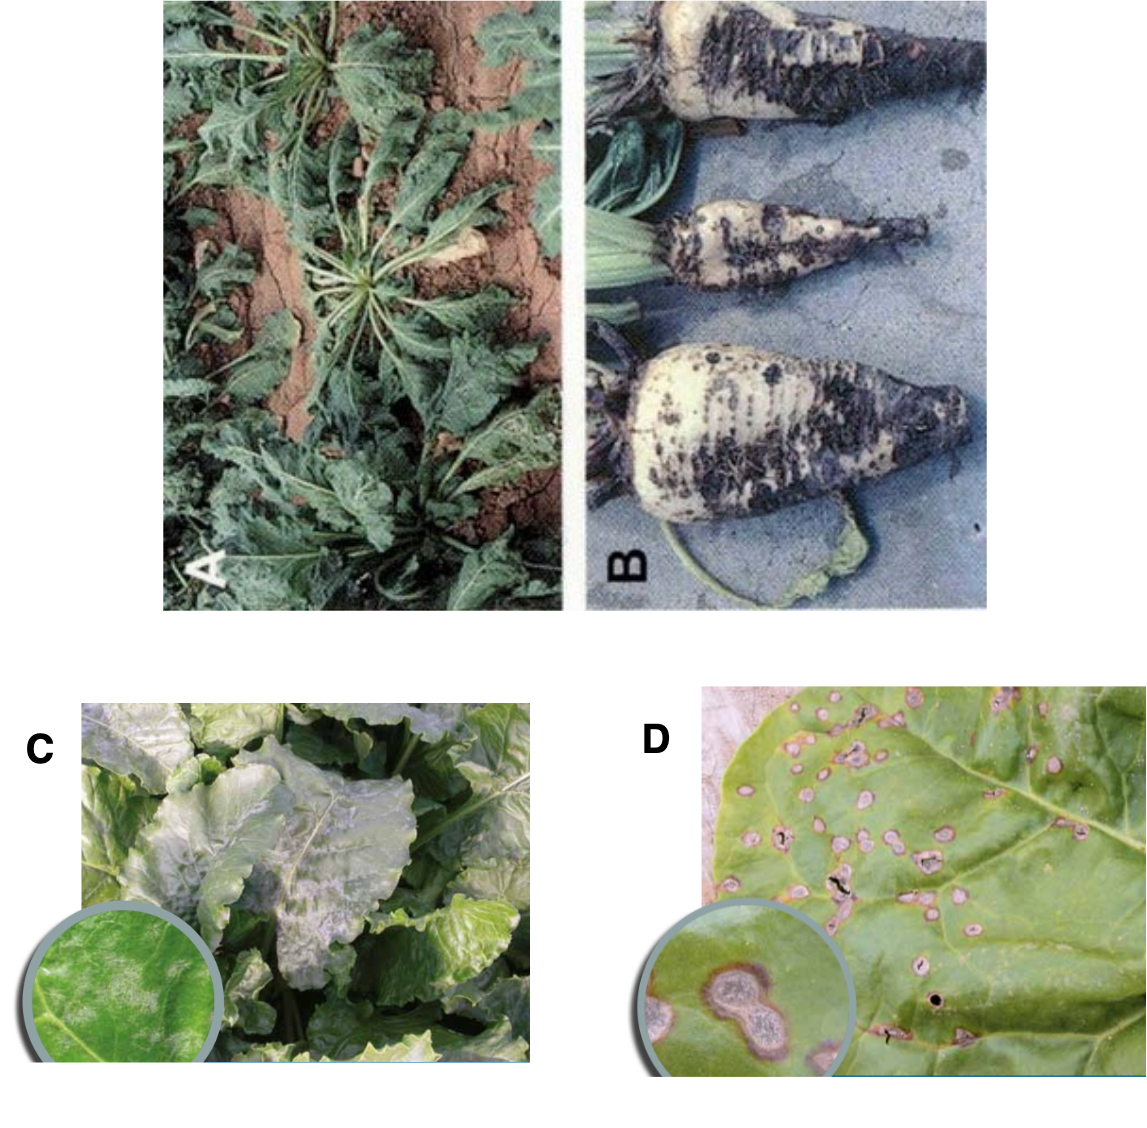
\includegraphics[scale=0.4]{figure/Untitled2.png}}
        \caption{(a,b) RCRR, (c) powdery mildew and (d) CLS disease in sugar beet \cite{articleHarveson}.}

        \label{fig:disease}
    \end{figure}




\chapter{Disease Assessment Sensors}\label{cha:acessDisease} 
Practical and less time-consuming monitoring of plant diseases is possible using image-based technologies like hyperspectral imaging, Red-Green-Blue (RGB) channel images, and spectroscopy. 
% RGB and hyperspectral imaging sensors are commonly used in research papers for non-invasive disease monitoring and detection.
In research papers, RGB and hyperspectral imaging sensors are usually used for non-invasive disease monitoring and detection. Section \ref{rgb} and \ref{hyperspectral} of the paper explains RGB and hyperspectral image-based technologies, respectively, including figures to give a visual explanation of each technique. In addition, the respective sections briefly review studies that used these sensors for disease detection. Finally, the chapter concludes with a summary of the discussed techniques found in research papers.

% ✅✅
% \item what is RGB image
\section{RGB Image}\label{rgb}
An RGB image is a coloured image with each pixel containing a particular red, green, and blue value based on the colour model. Each colour channel in the RGB image account for an 8-bit monochrome value per pixel out of the total 24-bit / pixel \cite{padmavathi2016implementation}. This means that each channel can take a value within the range of 0 up to 255.

The hue - the pure colour of the pixel without tint or shade - is the essential characteristic for differentiating between healthy and diseased plants from an RGB image in precision farming \cite{bock2010plant}. The colour information an RGB image holds allows for a conversion of the image into 14 different colour spaces possessing 86 various colour features \cite{shrivastava2015exploring}.

Moreover, using RGB images for plant disease detection relates to the conventional way of visually identifying plant disease based on colour changes to the leaves using the human eyes. The access to all the colour information of a plant captured by an RGB image 
 which is helpful for plant disease detection, mainly when used with machine learning models to allow for automatic detections \cite{shin2021deep}.
% ✅✅✅✅
% \item what is hyperspectral imaging. what is the wavelength?
\section{Hyperspectral Imaging}\label{hyperspectral}
Hyperspectral technology is a non-destructive and non-invasive detection technology that can obtain a large amount of narrow and continuous band spectral information from objects in the electromagnetic spectrum regions. Therefore, monitoring changes in the compositional structure of target objects is possible from the spectral data obtained by a hyperspectral imaging system.

Hyperspectral imaging (HSI) is the method of acquiring a hyperspectral image that contains an object’s spectral and spatial information as an image in 3-d stored in a spectral cube using a spectrograph coupled with a digital image sensor like CMOS or CMOS \cite{nguyen2021early, bock2010plant}. The structural and chemical changes that occur during plants reactions to disease pathogens have a direct influence on the reflectance spectra of plants leaves, which HSI can pick up; hence the reason for their usage in plant disease detection \cite{kuska2015proximal}. This capability makes HSI cameras vital in monitoring diseases in a sugar beet plantation since subtle differences in the spectral information of the leaves can be detected using HSI and could indicate an early detection of diseases in the plant.

Hence, with HSI, early detection of disease symptoms can be discovered using the spectral signatures of plant leaves and even soil-borne diseases \cite{kuska2015proximal, hillnhutter2010hyperspectral}. 
%The abundance of researches in plant disease detection using HSI is evidence of the strength and reliability of this technology for plant disease severity monitoring \cite{nagasubramanian2019plant, ochoa2016hyperspectral, yuan2019detection, moghadam2017plant}.

It is worthy to note that the range of wavelengths an HSI device can detect is dependent on the sensitivity range of the digital sensor device possesses, and also the spectral dispersion optics \cite{bock2010plant}. The bands of wavelengths documented in some plant disease detection researches are 400 nm - 2500 nm \cite{hillnhutter2011remote}, 400 nm - 1000 nm \cite{kuska2015proximal}.

\subsection*{Example Approaches}

% \begin{enumerate}


\item \cite{yones2019ajab} in their paper employed HSI to detect the infestation of Cotton leafworm, Aphid and Whiteflies diseases in a sugar beet plantation in the Minya governorate of Egypt. The study aimed at identifying the optimal spectral zone and spectral wavelength for detecting certain diseases in a sugar beet plant leaf. They used the hand-held ASD field spectrometer with a 350 - 2500 nm spectral range to acquire their spectral datasets. Twenty spectral image samples of the leaves were taken during the young and old sugar beet plant vegetative growth stages. Tukey’s HSD (honestly significant difference) test analysed and separated the datasets into healthy and unhealthy plant leaves. It was discovered that the blue (0.45-0.51$\mu$m) and NIR (Near Infrared 0.76-0.90$\mu$m) spectral zones were particularly successful in discriminating between healthy and unhealthy sugar beet plant leaves. Likewise, the blue spectral band showed remarkable results in further discriminating between the different disease infestations (Cotton leafworm, Aphid and Whiteflies) in infected sugar beet plants.
On the other hand, the paper used LSD (linear discriminant analysis) to identify the optimal wavelengths where different diseases are visible. The result of the LSD analysis showed that the SWIR (short wave infrared range) between 1500 and 2000 nm were optimal for identifying the three kinds of diseases mentioned above. Conclusively, they found out that the spectral discrimination of plant health was more visible in older plant leaves. 

\item Likewise, \cite{laudien2005multitemporal} used a supervised knowledge-based classification of hyperspectral vegetation index approach to differentiate between healthy and infected sugar beet plants from their spectral leaf image data obtained in the south of Germany. The leafs’ spectral data were captured using AVIS (Airborne Visible/Near-Infrared Imaging Spectrometer) and a tractor based GVIS (Ground-operated Visible/Near-Infrared Imaging Spectrometer) hyperspectral sensors. The AVIS hyperspectral sensor used can measure detailed spectral reflectance between 400 - 845 nm using 63 channels, a spectral interval of 9 nm, and a resolution of 4 metres. The GVIS sensor, on the other hand, is capable of measuring spectral reflectance between 380 - 860 nm by using 63 spectral channels. The hyperspectral measurement of the sugar beet plant leaves was taken with the two sensors for different intervals in 2003 (June, July, August and September). The study analysed and classified differences between healthy and unhealthy sugar beets plant datasets with a modified version of the Optimised Soil-Adjusted Vegetation Index (OSAVI) equation using ArcGIS 8.3 software. For the classification task, they used the result from the addition of the four OSAVI values obtained from the data acquisition campaign. The quantile classification method of ArcGis was used to classify the combined OSAVI values into nine vitality classes. The lower the class number, the healthier the sugar plant is. They found that $Rhizoctonia solani$ infected only 25\% of the sugar beet plantation field. They concluded that this low infestation detection percentage was attributed to the fact that there was no known $Rhizoctonia solani$ infestation on sugar beets in the research area in the year 2003 and the low spatial resolution of the captured datasets.

\item Also, \cite{hillnhutter2011remote} researched on the detection of stress-induced on a sugar beets plantation infested by $Heterodera schachtii$ and $Rhizoctonia solani$ using HSI sensors. The site used for the research is in Rheinbach, Germany. The field site was already infested with $Heterodera schachtii$ and $Rhizoctonia solani$. Therefore, they applied fertilisers and herbicides to the farmland before planting the Beretta variety of sugar beets. The researchers used Airborne Imaging Spectroradiometer for Applications (AISA, Oulu, Finland), a hand-held non-imaging spectroradiometer (ASD FieldSpec Pro Spectrometer, USA) and Hyperspectral Mapper (HyMap, Australia) imaging sensor for obtaining the spectral leaf data. AISA, ASD and HyMap can capture spectral data within the wavelength of 400 - 2500 nm, 400 - 1050 nm, and 450 - 2500 nm, respectively. AISA and HyMap provide 481 and 126 spectral bands, respectively, between their wavelengths. The 50 image samples obtained using AISA and HyMap were analysed using the Spectral Angle Mapper (SAM) classification method, with a split of 50\% as training and testing dataset. The SAM classification of AISA spectral image at week 31 of the planting season resulted in an accuracy of 72\%. Also, the week 39 spectral image from the plantation season achieved an accuracy of 64\% in classifying the sugar beet plant health. They concluded that despite the inconsistencies in the detection by the different HSI sensors, using canopy reflectance for monitoring disease in sugar beet is a promising approach to take.

% \end{enumerate}



\begin{table}[h!]
\centering 
 \begin{tabular}{p{3cm}|p{2cm}|p{2.5cm}|p{2cm}|p{2cm}|p{2cm}} 
 
%   \begin{tabular*}{\textwidth}{|c|c|c|c|c|c|}
%   \begin{tabular*}{\textwidth}{c @{\extracolsep{\fill}} c @{\extracolsep{\fill}} cccc}

% \begin{tabular}{p{0.2\textwidth}p{0.2\textwidth}p{0.2\textwidth}p{0.2\textwidth}p{0.2\textwidth}p{0.2\textwidth}}
 \hline
  Sensor & Wavelength & Algorithm & Accuracy & Field site & Reference\\ [0.5ex] 
 \hline\hline
 hand-held ASD field spectrometer & 350 - 2500 nm & HSD Tukey \& LSD & - & Minya, Egypt& \cite{yones2019ajab} \\ 
 \hline
 AVIS \& GVIS spectrometer & 400 - 845 nm \& 380 - 860 nm & quantile method classifier / OSAVI & - &South Germany& \cite{laudien2005multitemporal} \\ 
 \hline
  AISA, hand-held ASD field spectrometer \& HyMap spectrometer & 400 - 2500 nm, 400 - 1050 nm, \& 450 - 2500 nm & SAM classifer & AISA 72\%, HyMap 54\% & Rheinbach, Germany & \cite{hillnhutter2011remote} \\ 
 \hline
 \end{tabular}
 \caption{ Overview of hyperspectral imaging methods for discriminant disease detection in Sugar beet.}
 \label{table:1}
\end{table}

\FloatBarrier

Overall, it can be concluded that using HSI sensors for the non-invasive health monitoring of sugar beets has shown great potential for discriminant disease detection. Table \ref{table:1} shows the HSI sensors, wavelengths, and algorithm used to monitor sugar beet plants’ health in the reviewed research papers.



\chapter{Analysis}\label{cha:Analysis}
% \section{Analysis}

Different non-invasive approaches for leaf disease detection have been developed, and the application of Machine learning algorithms on image datasets from various sensors are gaining traction \cite{ferentinos2018deep, ahmed2019rice, annabel2019machine, ramesh2018plant}. A typical learning-based approach workflow consists of input datasets acquisition, data pre-processing, model training, model evaluation and finally, deployment. Feature extraction, segmentation, and region detection are data pre-processing steps for image datasets. This chapter starts with a brief explanation of the Convolutional Neural Network (CNN) in deep learning in section \ref{sec:machinedeep}. Then, the paper further reviews different machine learning and deep learning techniques used in research papers to detect different diseases in sugar beet leaves in section \ref{sec:deeplapproach} and \ref{sec:machineapproach}, respectively.

% ✅✅✅
\section{Machine Learning and Deep Learning}\label{sec:machinedeep}
Machine learning is a sub-field of artificial intelligence that enables computers to create a mathematical model of raw data using mathematical algorithms to extract relevant patterns for prediction or classification tasks. Machine learning models are classified into three categories depending on the level of human intervention on the input dataset; supervised, unsupervised and reinforcement learning. In a supervised learning approach, the algorithm makes predictions based on the discovered correlation between the features in the input dataset and the expected outcome (label) present in the dataset. In Unsupervised learning, the algorithm recognises patterns and relationships in the unlabelled input dataset itself. Finally, reinforcement learning is reward-based learning. The algorithm learns from the negative or positive feedback it gets for making decisions on datasets. K-nearest neighbours, Naive Bayes, logistic regression, decision tree, and support vector machines (SVM) are machine learning algorithms for classification tasks \cite{goodfellow2016deep}.

In contrast, Deep learning (DL) is a learning strategy based on a neural network that empowers computers to learn and advance through encounters with data channelled through diverse handling layers of artificial neural network architectures. In other words, Deep learning techniques are a computational model of how learning occurs in the human brain \cite{goodfellow2016deep}.
The neural network structure often consists of an input layer, one or many hidden layers, and finally, an output layer. Figure 2 gives an overview of the general framework of Deep learning. Some of the common constituents of any DL architecture are convolutions, pooling layers, fully connected layers, activation functions, memory cells, bias, weights, transfer function, amongst others \cite{goodfellow2016deep}. The types of neural network architectures in DL includes recurrent neural network (RNN), recursive neural network, convolutional neural network (CNN), generative adversarial network (GAN), and Multi-Layer Perceptron (MLP)\cite{nielsen2015neural}. Out of these networks, CNN is often used in precision farming for plant disease classification because of its success in the categorisation of objects with minimal pre-processing of input data \cite{sardogan2018plant}.

Interest in the use of CNN began when Geoffrey Hinton, Ilya Sutskever, and Alex Krizhevsky won the 2012 ImageNet Large Scale Visual Recognition Competition (ILSVRC) with a model trained using CNN architecture \cite{russakovsky2015imagenet}. Ever since then, different variations of CNN based models have evolved for the task of image classifications. Some of the very deep CNN architectures are AlexNet, GoogleNet, VGGNet, Inception ResNet, just to mention a few \cite{szegedy2013intriguing, simonyan2014very, szegedy2017inception}. A typical CNN architecture is made up of several stacks of layers. The initial layer is the convolutional layer, followed by pooling, activation, and fully connected layers.

The convolution layer takes care of extracting feature maps through mathematical calculations with weights and kernel - filters - as the input image is scanned through. 
In the pooling layer, the size of the feature map from the previous layer is reduced by only keeping one representation of the values in a region. Typical approaches to pooling are max pooling and average pooling. Maximum pooling takes the maximum value in the specified region, while average pooling takes the average of the values in the neighbourhood.
The extracted feature map is then passed through an activation function that ensures no linearity in the network. Rectified linear unit (RELU) and sigmoid are typical examples of this function. Finally, the fully connected layer classifies the output from the activation layer. Therefore, the output of the fully connected layers is the different classifications the architecture could make.

Besides, some of the advantages of DL over traditional ML techniques are the automatic feature extraction, ability to understand the compositional hierarchies of data and increase in the complexity of models, which results in faster runtime or reduced time complexity and increased classification accuracy \cite{kamilaris2018deep}.

However, a Faster region convolution neural network (Faster R-CNN) is a CNN based architecture used for object detection. It is an advancement over the previous computationally expensive R-CNN and Fast R-CNN \cite{ren2015faster}. Object detection aims to detect instances of objects of interest in an image. To achieve the detection task on an image, search algorithms like the selective search algorithm is used to extract around 2000 region proposals from the input image, which are then fed into CNN for proper feature extraction\cite{girshick2014rich}. The extracted features are then classified into regions using SVM. This approach is called R-CNN. However, this approach was found to be slow in object detection and computationally expensive to train \cite{girshick2015fast}. As an improvement over R-CNN, R. Girshick (the inventor of R-CNN) introduced Fast R-CNN. The fast R-CNN architecture feeds both the input image and set of object proposals together into the neural network \cite{girshick2015fast}. After extracting the feature map, the region of interest is reshaped to fixed sizes using the ROI pooling layer. The network’s output is the probability of the proposed region’s class and the predicted class’s refined bounding-box position.
Still, Fast R-CNN was found to be limited in real-time object detection \cite{zou2019object}.
As a further improvement over R-CNN and fast R-CNN, Faster R-CNN was introduced \cite{ren2015faster}. The significant difference of faster R-CNN over other previous architectures is using a separate region proposal network to identify the object detection region proposal. In addition, using RPN significantly reduced the computational cost of training and testing on datasets \cite{ren2015faster}.

\section{Deep Learning Example Aprroaches}\label{sec:deeplapproach}
\begin{enumerate}
\item Ozguven and Adem \cite{ozguven2019automatic} in their paper examined the automatic detection and classification of leaf spot disease in sugar beet plants using deep learning algorithms. In total, 155 RGB images were trained and tested using Faster R-CNN and their proposed updated Faster R-CNN architectures with 150 000 iterations amounting to a training time of 30 hours. Of the 155 images, 38 were healthy, 20 had mild disease, 35 were severe, and 62 were mild and severe diseased in mixed proportions.
Their research trained the Faster R-CNN model using 32 different 3 x 3 filters with 1 for the value of stride and padding on a 32 x 32 x 3 input image size. On the other hand, they trained their proposed updated Faster R-CNN using 64 different 3 x 3 filters with 4 for the value of stride and 2 for the value of padding on a 600 x 600 x 3 input image size, increasing the input image size aimed at trying to increase the possibility of identifying non-prominent diseased areas. They increased both the value of the stride and padding to avoid additional computational responsibilities that come with an increase in the image size and number of filters. In training and testing both models, they used 85\% randomly selected portions of the 155 sugar beet leaf images for training and the rest for testing. However, it is unclear under what condition the datasets were obtained. They trained for 150 000 iterations using Matlab 2017b for windows. Upon evaluating results from both models, they realised that the Updated Faster R-CNN model performed better in detecting the diseased section of sugar beets leaf with an overall accuracy of 95\%.
In contrast, the Faster R-CNN model had an accuracy of 92.89\%. Nevertheless, their proposed updated Faster R-CNN model incorrectly classified six images of sugar beet leaf as healthy and one image as diseased. These misclassifications were due to shadows over the sugar beet leaf images. Unfortunately, they could not compare their results with other research work on leaf disease detection in sugar beet using deep learning since they were the first to do such.

\item In other related studies of plant leaf disease detection with CNN architectures, Authors in \cite{sujatha2021performance} used 609 citrus plant leaf RGB images for the classification of four citrus leaf diseases - Blackspot, Melanose, Canker and Greening disease - present in their dataset using both machine learning and deep learning methods. They aimed at finding the best classifier between these methods in disease detection. They discovered that the deep learning architecture used  VGG-19, VGG-16, and Inception-v3, with an accuracy of 87.4\%, 89\%, and 89.5\%, respectively, to perform better than machine learning algorithms used in detecting disease in citrus plant leaves. On the other hand, the machine learning algorithms  RF, Stochastic gradient descent and SVM had 76.8\%, 86.5\% and 87\% accuracy.

\item Likewise, Ferentinos \cite{ferentinos2018deep} in his study developed CNN based models for automatic plant disease detection and diagnosis system from images of plant leaves. The study trained models on 87 848 pictures of healthy and diseased 25 different plant leave from an open-source database consisting of experimental laboratory images and actual cultivation conditions photos. In the studies, the most successful model trained with VGG architecture achieved an impressive accuracy of 99.53\% in the classification of unseen 17 548 plant leaves images. However, despite a high accuracy rate, the paper concluded that the model is still quite far from being used in natural cultivation conditions due to different geographic, cultivation and image capturing conditions, which might render the trained model unstable.
\end{enumerate}

\begin{table}[h!]
\centering 
 \begin{tabular}{p{2cm}|p{2cm}|p{2cm}|p{2cm}|p{2cm}|p{2cm}} 
%   \begin{tabular}{|c|c|c|c|c|}
 \hline
  Sensor & No. of Images Used  & Model & Training Time & Accuracy & Reference\\ [0.5ex] 
 \hline\hline
 RGB imaging & 155 & Faster R-CNN & 30 hours & 92.89\% & \cite{ozguven2019automatic} \\ 
 \hline
 RGB imaging & 609 & VGG-19, VGG-16, Inception-v3 & - & 87.4\%, 89\%, 89.5\% & \cite{sujatha2021performance} \\ 
 \hline
  RGB imaging & 87 848 & VGG & - & 99.53\% & \cite{ferentinos2018deep} \\ 
 \hline
 \end{tabular}
 \caption{Overview of CNN learning-based papers for leaf disease detection tasks.}
 \label{table:2}
\end{table}

\section{Machine Learning Example Approaches}\label{sec:machineapproach}
\begin{enumerate}
\item Barreto et al. \cite{Barreto2020HyperspectralIO} in their studies researched on the use of machine learning and non-invasive sensors for early detection and measuring the incidence of disease in sugar beets. They cultivated the Sabrina cultivar variety of sugar beet susceptible to Rhizoctonia root and crown rot (RRCR) under controlled conditions for their research. A total of 50 sugar beet plants were planted for this research. They inoculated the plants with $R.solani$ at week 8 of cultivation. The datasets used for training the machine learning algorithms were acquired at eight different time points before and after disease injection into the plants. The Hyperspectral image datasets were captured in a controlled laboratory environment using the Hand-held VIS-NIR sensor(Oulu, Finland) with a spectral reflectance range between 400 - 1000 nm. They calibrated the raw image with Specim IQ Studio software, obtained the hypercube with 68 channels, reduced random noises with Savitzky–Golay filtering and extracted region of interest (ROI). Their pre-processing stage resulted in a hyperspectral image with 557 channels. All fifty plants and their respective spectral information and visual rating were randomly split into three sets. 40\% of the dataset was used to train the machine learning models, 40\% to test the trained models, and the remaining 20\% to analyse the effect of reduction in spectral information using recursive feature elimination (RFE). The authors trained the machine learning model with k-nearest neighbours (KNN), the partial least squares (PLS), the random forest (RF), the support vector machine linear (SVML) and the support vector machine radial (SVMR). The RFE algorithm identified 19 wavelengths as most important for the detection of RRCR. Out of the five machine learning techniques used in the study, the model trained with RF performed the best. The RF model achieved its best results on the datasets from 10 to 17 days after inoculation. It was also discovered that their RFE classifier performed 50\% better in classifying infected plants than the human eye. Furthermore, they were able to conclude based on the results of their research on the possibilities of early RRCR disease detection in sugar beet using the information from leaf reflectance.

\item Hallau et al. \cite{hallau2018automated} presented an SVM learning-based approach for the detection and identification of 5 sugar beet leaf diseases using RGB-image captured with a smartphone’s camera. The sugar beet diseases distinguished in this paper are CLS, Ramularia leaf spot (RLS), Phoma leaf spot (PLS), beet rust and bacterial blight. The research used images captured by Samsung GT-I9300 (Samsung Electronics GmbH), a Sony Ericsson LT18i (Sony Mobile Communications AB) and a Motorola DEFY + (Motorola Inc.) under controlled and field conditions in Kerpen, Germany. The experiment used more than 48 different sugar beet cultivars susceptible to leaf diseases. The database included symptom images of five-leaf diseases of sugar beet as well as images of healthy leaves and comprised non-diseased leaves (450 images), CLS (720), RLS (200), PLS (30), beet rust (220) and bacterial blight (250). In preparing the image for the machine learning detection task, the raw input image was down-scaled by 25\% to increase sharpness and the brownish/reddish regions in the raw input image were highlighted. Then, using the extracted regions, feature computation using texture features and classification on computed features with a multi-class SVM using the radial basis function (RBF) kernel were done. In total, the classifier algorithm was trained on six classes, with the 6th class being the non-diseased leaf images for evaluating the model. As a result, they averaged 93.1\% and 94.6\%, classifying a plant as diseased or otherwise by training their model on 495 images containing 269 and 2957 extracted regions, respectively. Likewise, they averaged 83.7\% and 75.2\% in the multi-class disease classification using the same 495 images with their extracted regions. Major misclassifications were attributed to the shortage of sufficient extracted regions of PLS and RLS in the datasets due to their rare occurrence in Germany.
As proof of the adequacies and authenticity of their trained model, they compared trained machine learning models with 27 experts in the sugar beet field who evaluated 30 hand-picked images from the datasets. 46.4\% was the overall accuracy of the experts’ predictions. They also discovered that the bacterial blight, CLS, and RLS proved difficult for the experts’ to differentiate. Compared with other research, their disease detection method was less computationally expensive and performed better in disease detection and classification, although the images were collected under less defined conditions.


\item Zhou et al. \cite{zhou2013early} proposed a novel framework for early detection and continuous quantisation of CLS in sugar beet by combining the template matching method of orientation code matching (OCM) with the machine vision method of SVM. The research used the Amaibuki sugar beet cultivar planted and infected under controlled conditions in Japan for the experiment. 2144 x 1424 resolution RGB images of the plants captured using Nikon D300 (NIKON Co., Japan) digital camera was used for the classification task. 
The paper used an extended version of OCM to dynamically track site-specific and continuous observation of disease development identical leaf parts from time sequence images against illumination using a 50 x 50 pixels search window. Likewise, segmentation of the plant leaves is done using the G-R segmentation factor to distinguish leaf parts from the soil background automatically. Then the xy-colour histogram feature is used for training the SVM classification model to segment the disease pixels from healthy and their background pixels based on extracted features. They achieved 96.52\% and 99.47\% classification accuracies from their trained model using training and testing samples, respectively. They concluded that their proposed approach could be used in a cultivated field under natural lighting conditions for early and continuous detection of CLS in sugar beet.

\item Ziya et al. \cite{ziya34determination} in their study researched the efficiency of using machine learning algorithms to determine the level of CLS disease in sugar beet leaves compared to visual assessments done by experts. The sugar beet field used for the study is located in Tokat province of Turkey. The RGB images of the leaves were captured between August and September 2016 using DJI Phantom 3 drone and pre-processed using MATLAB R2014a. The authors trained their algorithm with 12 leaf images with varying CLS infection levels taken at distances between 30-60 cm from the drone and plants under natural lighting field conditions at 4000 X 2250 pixel resolution. Initially, the captured RGB images were converted to L*a*b colour space. Then, the colours in the a*b* region that signify disease image pixels were classified using the k-means clustering algorithm. Then each pixel of the image is tagged using the results from the k-means clustering. The disease leaf image is then colour separated according to their pixel tags. Finally, after enhancing the contrast of the colour image, the processed image is converted back to RGB colour space containing the information of the identified disease areas. Figure \ref{fig:k_clusterd} shows the resulting image from the steps described above. The brown segments in the last image of figure \ref{fig:k_clusterd} are the infected areas on the leaf.  The severity of infestation caused by CLS in the clustered image is calculated by dividing the number of diseased pixels by the total number of pixels in the leaf image. The result obtained using their techniques showed an accuracy close to that obtained by visual observations of experts. This proximity in results signified that the proposed method could be used for disease monitoring even under natural lighting conditions as long as the drone’s height is within 60 cm from the plants.


    \begin{figure}[htbp]
        \centerline{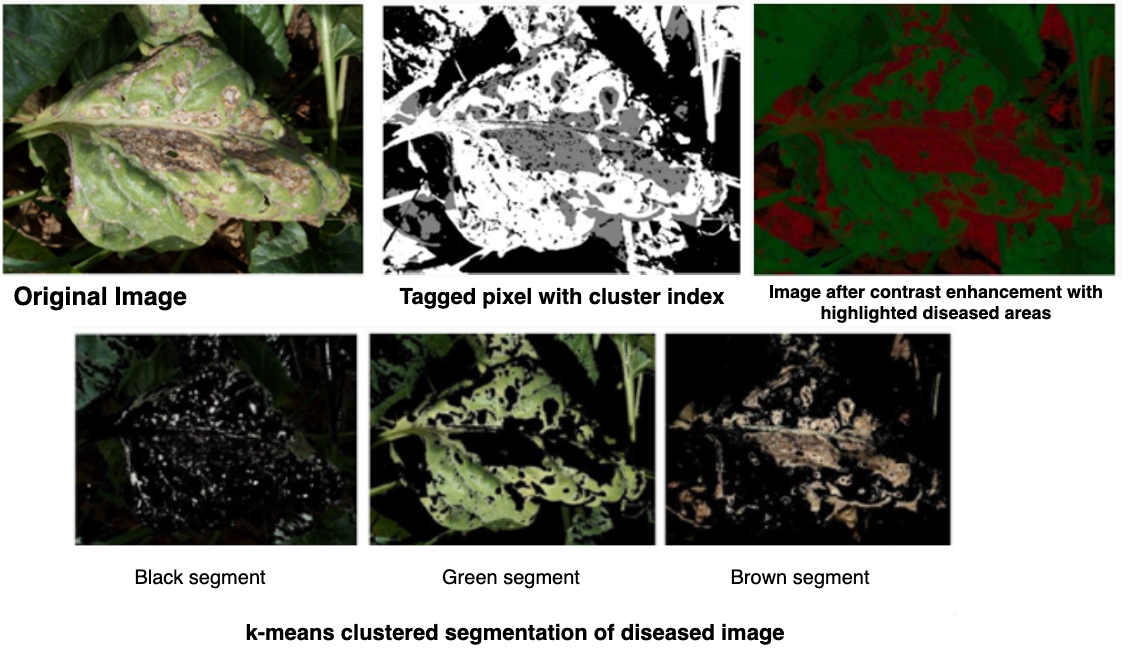
\includegraphics[scale=0.32]{figure/Untitled.png}}
        \caption{Resulting image of each steps in the proposed techniques described in \cite{ziya34determination}.}

        \label{fig:k_clusterd}
    \end{figure}


\item Bauer et al. \cite{bauer2011potential} in their paper researched the potential of using  KNN and adaptive Bayes with GMM pixel-wise algorithms to classify leaf disease in sugar beets automatically. They also investigated the use of conditional random fields (CRF) global labelling approach to improving pixel-wise-based classification results. Their classification task had three classes: $healthy \thinspace leaf \thinspace area$, $Cercospora \thinspace beticola$, and $Uromyces \thinspace betae$. For their experimental purpose, the authors inoculated 15 plants with the leaf spot pathogen $Cercospora \thinspace beticola$ and another 15 plants with the rust fungus $Uromyces \thinspace betae$. For each of the four leaves in each plant, they took 4 RGB images (FujiFilm FinePix S5600, 2592 x 1944) and one multispectral image (Tetracam ADC, 1280 x 1024, wavelength 700 - 950 nm) from a height of 30 cm and at different positions separated by about 10 cm. Then, they fused the five images of each leaf into one image representing the 3-D structures of the combined leaves’ to allow for rectification. The rectification of the 3-D image resulted in a 15-channel 2-D image. From these 15 values, they used only one blue, one green and one red value from one of the RGB images and the infrared channel from the multispectral image as classification features. They selected image patches that showed only healthy and infected leaf areas with no background for training and testing their models. From the resulting image patches, they chose 350 randomly for both diseases so that the test dataset finally contained 700 image patches. Also, in training their kNN classifier, they performed two experiments. The first experiment trained using four colour information from a particular pixel and the other using neighbouring pixels. For each experiment, they randomly chose 2000 pixels from half of the  700 image patches in the test dataset for training, and the other half was used for testing purposes. This was done to reduce the training computation time, and the kNN training and testing were done five times for each experiment. Likewise, They trained their adaptive Bayes classification models using Gaussian mixture models. 1 in 10 of the 700 image patches was randomly selected and used their complete information for training.
The trained model was then tested on the remaining 630 image patches. Thus, the GMM model training and testing were done ten times. Their kNN classifier achieved median accuracies of 84\%, 74\%, and 59\% for the $healthy \thinspace area$, $Cercospora \thinspace beticola$ and $Uromyces \thinspace betae$ respectively from the first experiment. In contrast, the median classification achieved in the second experiment were 91\%, 81\% and 76\% for the $healthy \thinspace area$, $Cercospora \thinspace beticola$ and $Uromyces \thinspace betae$ respectively. Likewise, the median accuracies for GMM trained models were 94\% for the $healthy \thinspace leaf \thinspace area$, 91\% for $Cercospora \thinspace beticola$ disease and 91\% for $Uromyces \thinspace betae$ disease. Finally, their CRF experiments concluded that it is possible to improve the result of an independent pixel-wise classifier with a global smoothing model. Likewise, their best classifier (GMM) results concluded that differentiating between healthy and infected sugar beet leaves is possible.
\end{enumerate}

\begin{table}[h!]
\centering 
 \begin{tabular}{p{2cm}|p{2cm}|p{2cm}|p{2cm}|p{2cm}|p{2cm}} 
%   \begin{tabular}{|c|c|c|c|c|}
 \hline
  Sensor & Wavelength & No. of Images Used & Model & Overall Accuracy & Reference\\ [0.5ex] 
 \hline\hline
 hand-held VIS-NIR spectrometer & 400 - 1000 nm & 50 & KNN, PLS, RF, SVML, SVMR & -  & \cite{Barreto2020HyperspectralIO} \\ 
 \hline
 RGB imaging (Smartphones) & - & 495 & SVM & 94.6\% & \cite{hallau2018automated} \\ 
 \hline
 RGB imaging (Nikon D300) & - & - & SVM & 99.47\% & \cite{zhou2013early} \\ 
 \hline
  RGB imaging (DJI Phantom 3) & - & 12 & KNN & - & \cite{ziya34determination} \\ 
 \hline
  RGB imaging (FujiFilm FinePix S5600) \& multispectral imaging (Tetracam ADC) & 700 - 950 nm & 700 & KNN, GMM & 91\%, 94\% & \cite{bauer2011potential} \\ 
 \hline

 \end{tabular}
 \caption{Overview of researches using machine learning algorithms for leaf disease detection in sugar beet.}
 \label{table:3}
\end{table}

\FloatBarrier

The studies in this chapter explored non-invasive leaf disease detection techniques in sugar beet with different ML and DL learning-based approaches. These studies demonstrate that sugar beet plant leaves can be monitored and classified as healthy or infected based on hyperspectral and RGB imaging data. Table \ref{table:2} shows an overview of the key metrics in the reviewed machine learning-based research papers, while table \ref{table:3} shows CNN learning-based approaches. The hyperspectral images provide spectral information that enables disease detection using learning-based algorithms. In contrast, the colour channels in RGB images give enough information for leaf disease detection and classification tasks.
    
   



\chapter{Conclusion}\label{cha:conclusion}
This paper reviewed studies done in the area of non-invasive leaf disease monitoring and detection in sugar beets. First, the paper discussed the causative agents, signs and symptoms of three common diseases that affect the quantity and quality of yields in a sugar beet plantation season in Chapter \ref{cha:Fundamentals}. Second, Chapter \ref{cha:acessDisease} of the paper presented the hyperspectral and the RGB imaging sensors for capturing information from plant leaves in section \ref{rgb} and \ref{hyperspectral}. Furthermore, the sections explored different researches that used hyperspectral imaging for leaf disease detection tasks. Third, the paper gave an introduction to machine learning and CNN in Chapter \ref{cha:Analysis}. Then the remaining sections examined different research papers that conducted studies using machine learning and CNN algorithms by citing their techniques for data capturing, pre-processing, training algorithms and accuracies.

While there are researches in the direction of using machine learning algorithms for leaf disease detection and monitoring in sugar beets, the feature extraction from datasets are dependent on human intervention, as evidenced in the studies reviewed in this paper. However, there are currently not enough researches exploring a deep learning-based approach for leaf disease detection in sugar beet. Therefore, more research needs to be done in this area since CNN-based architectures can automate the feature extraction process in a given dataset, reducing the human intervention needed. Likewise, more research needs to be carried out using datasets captured in field environments under different lighting and atmospheric conditions since the trained models are to be used in field environments, not in controlled laboratory settings common in research papers.



%Literaturverzeichnis
\newpage
\lhead{}
\rhead{\leftmark}
\addcontentsline{toc}{chapter}{References}

\bibliography{References}
\bibliographystyle{alpha}


\listoffigures				%Verzeichnis aller Bilder
\listoftables				%Verzeichnis aller Tabellen
%list of definitions, ...

\chapter*{Affidavit}
I \myauthor herewith declare that I have composed the present paper and work by myself and without use of any other than the cited sources and aids. Sentences or parts of sentences quoted literally are marked as such; other references with regard to the statement and scope are indicated by full details of the publications concerned. The paper and work in the same or similar form has not been submitted to any examination body and has not been published. This paper was not yet, even in part, used in another examination or as a course performance.
. ~\\
Lippstadt,  \today\\[.6cm] %<city>, <date>
\myauthor\\ % signature
\rule[0.5em]{20em}{0.5pt}

\appendix

\include{cha/08Appendix}

\end{document}
